\input{../YKY-preamble.tex}
% \usepackage[no-math]{fontspec}
% \setmainfont[BoldFont=Alibaba_Sans_Regular.otf,ItalicFont=Alibaba_Sans_Light_Italic.otf]{Alibaba_Sans_Light.otf}

\usepackage[backend=biber,style=authoryear]{biblatex}
\bibliography{../AGI-book}
\renewcommand*{\bibfont}{\footnotesize}

\usepackage[active,tightpage]{preview}		% for continuous page(s)
\renewcommand{\PreviewBorder}{0.5cm}
\renewcommand{\thempfootnote}{\arabic{mpfootnote}}

\usepackage[absolute,overlay]{textpos}		% for page number on upper left corner

\usepackage{color}
% \usepackage{mathtools}
% \usepackage[hyperfootnotes=false]{hyperref}
\usepackage{hyperref}

\usetikzlibrary{shapes}
% \usepackage[export]{adjustbox}	% ??
\usepackage{verbatim} % for comments
% \usepackage{newtxtext,newtxmath}	% Times New Roman font

% \titleformat{\subsection}[hang]{\bfseries\large\color{blue}}{}{0pt}{}
% \numberwithin{equation}{subsection}

\newcommand{\underdash}[1]{%
	\tikz[baseline=(toUnderline.base)]{
		\node[inner sep=1pt,outer sep=10pt] (toUnderline) {#1};
		\draw[dashed] ([yshift=-0pt]toUnderline.south west) -- ([yshift=-0pt]toUnderline.south east);
	}%
}%

\newcommand\reduline{\bgroup\markoverwith{\textcolor{red}{\rule[-0.5ex]{2pt}{0.4pt}}}\ULon}

%\DeclareSymbolFont{symbolsC}{U}{txsyc}{m}{n}
%\DeclareMathSymbol{\strictif}{\mathrel}{symbolsC}{74}
%\DeclareSymbolFont{AMSb}{U}{msb}{m}{n}
%\DeclareSymbolFontAlphabet{\mathbb}{AMSb}
%\setmathfont{lmroman17-regular.otf}
\DeclareMathOperator*{\argmin}{arg\,min}
\DeclareMathOperator*{\argmax}{arg\,max}

% \usepackage[most]{tcolorbox}
%\tcbset{on line,
%	boxsep=4pt, left=0pt,right=0pt,top=0pt,bottom=0pt,
%	colframe=red,colback=pink,
%	highlight math style={enhanced}
%}
%\newcommand{\atom}{\vcenter{\hbox{\tcbox{....}}}}

\let\oldtextbf\textbf
\renewcommand{\textbf}[1]{\textcolor{blue}{\oldtextbf{#1}}}

\newcommand{\logic}[1]{{\color{violet}{\textit{#1}}}}
\newcommand{\underconst}{\includegraphics[scale=0.5]{../2020/UnderConst.png}}
\newcommand{\KBsymbol}{\vcenter{\hbox{\includegraphics[scale=1]{../KB-symbol.png}}}}
\newcommand{\token}{\vcenter{\hbox{\includegraphics[scale=1]{token.png}}}}
\newcommand{\proposition}{\vcenter{\hbox{\includegraphics[scale=0.8]{proposition.png}}}}
\renewcommand\sigmoid{\vcenter{\hbox{
\includegraphics{sigmoid.png}}}}

\begin{document}

\begin{preview}

% \noindent {\color{cyan}``\textit{If men cease to believe that they will one day become gods then they will surely become worms.}''
% \hfill --- Henry Miller}

\cc{
\title{\vspace{-0.5cm} \bfseries\color{blue}{\Huge 「绳子戏法」 \normalsize -- 人工智能的数学}}
}{
\title{\vspace{-0.5cm} \bfseries\color{blue}{\Huge String Diagrams}}
}

\author{\small YKY [\today]} % Your name
\date{\vspace{-0.5cm}} % Date, can be changed to a custom date
% \date{\small \today}

\maketitle

\setcounter{section}{-1}
\newcounter{mypage}
\setcounter{mypage}{0}

% (1) Circled page number on upper left corner
%\begin{textblock*}{5cm}(2.1cm,2.3cm) % {block width} (coords)
%{\color{red}{\large \textcircled{\small \themypage}}}
%\addtocounter{mypage}{1}
%\end{textblock*}

\begin{minipage}{\textwidth}
\setlength{\parskip}{0.4\baselineskip}

最近经常讲政治，如果不进一点人工智能，大家可能觉得我是冒牌货了。今次进一种叫 string diagrams 的东西，它是我近来最有趣的发现，也跟我研究的突破密切有关。

事情开始于考虑逻辑的 \textbf{对称性结构}，例如 \textit{我爱你 $\neq$ 你爱我}，但 \textit{我爱你 $\wedge$ 你爱我 = 你爱我 $\wedge$ 我爱你}。 这是一种叫 \textbf{交换性} 的对称。 而大家应该也听过，作为现代 LLM 最基本元件的 Transformer 也有这种交换对称性。 于是就有令我很兴奋的猜测： 会不会 Transformer 就暗藏逻辑的结构呢？ 但事与愿违，Transformer 结构 跟逻辑结构 总是对不上。 Transformer 将句子 拆成 tokens，例如「我」、「爱」、这样的一些原子概念，而 tokens 是可交换的。 但 \textit{我爱你 $\neq$ 你爱我} 是 \textbf{不可交换}。 于是，单词 似乎不对应 tokens，但如果 句子/命题 对应一个 token，则它又可以分拆为更小的单位。 总之，好像逻辑结构 对不上 Transformer 结构。

后来我开始研究 \textbf{对称性} 是怎样用 神经网络 实现（当然，其实只是其他人的研究成果，我在学习）。 Kolmogorov-Arnold 给出了 对称函数的一般 \textbf{代数形式}： $f(x_1, ..., x_n) = g( h(x_1) + h(x_2) + ...)$.  显然，\textbf{加法} 是有交换性的，而这个定理告诉我们，所有对称函数其实都可以用这种加法结构实现\footnote{这个定理的证明其实颇为复杂，我看了两个截然不同的证明，都勉强看懂了，但完全想不出他们是怎样想出那些证明的。可以参看 DeepSet 和 PointNet 的论文。}。 但我直接用这种神经网络做逻辑推理，效果却不太理想。

于是又回到 Transformer. 它也有对称性，但这种对称性是用 dot product 和某些 matrix 运算 巧妙地达成的 （图 \ref{eqn:attention-string-diagrams} 的左下角 就是著名的 Self-Attention 公式，亦即 Transformer 的结构），它不是根据什么定理。 我想了解这些运算 \textbf{为什么} 达成了对称性，而我直觉觉得 它可能跟 string diagrams 有关。

\begin{equation}
\begin{aligned}
\label{eqn:attention-string-diagrams}
% \hat{x}^k \mathrel{:}= \underset{\substack{i \in \text{predicates} \\
%	j \in \text{arguments}}}{\mathlarger{\forall}} \; \left\langle \mathrm{soft}\max_{ij} w_{ij}^k \; , \; x_{ij} \right\rangle
Z \mathrel{:}= \sigmoid \check{W} \otimes \left( \sigmoid \hat{W} \otimes X \right)
\qquad
\def \globalscale {0.4}
\vcenter{\hbox{\begin{tikzpicture}[y=1pt, x=1pt, yscale=\globalscale,xscale=\globalscale, every node/.append style={scale=\globalscale}, inner sep=0pt, outer sep=0pt]
	\begin{scope}[shift={(-115.59316, 283.87838)}]
		\path[draw=black,line width=0.8pt] (137.10858, -254.31339) -- (358.01601, -254.31339);

		\path[draw=black,line width=0.8pt] (137.32536, -153.20368) -- (244.69474, -153.20368).. controls (320.66437, -152.86162) and (318.7147, -271.01124) .. (245.63945, -271.5473) -- (186.27009, -271.5473);

		\path[draw=black,line width=0.8pt] (358.69474, -222.80075) -- (137.60239, -222.80075);

		\path[draw=black,line width=0.8pt] (137.93392, -204.9619) -- (222.34139, -204.9619).. controls (231.27231, -204.9619) and (238.46219, -197.77202) .. (238.46219, -188.8411) -- (238.46219, -187.64698).. controls (238.46219, -178.71606) and (231.27231, -171.52618) .. (222.34139, -171.52618) -- (138.21151, -171.52618);

		\path[draw=black,line width=0.8pt,->] (238.40059, -188.98504) -- (252.76995, -188.98504);

		\path[draw=black,line width=0.8pt,->] (301.05457, -209.88868) -- (315.42393, -209.88868);

		\path[draw=black,line width=0.8pt] (137.32536, -271.70366) -- (181.69471, -271.70366);

		\path[draw=black,fill=white,line width=0.8pt] (196.87486, -259.50278) -- (196.87486, -283.50282) -- (177.37495, -271.5028) -- cycle;

		\path[draw=black,fill=white,line width=0.8pt] (198.11309, -159.66386) -- (198.11309, -183.6639) -- (178.61318, -171.66388) -- cycle;

		\node[text=black,scale=2.8] at (123.30065, -158) {$\hat{W}$};
		\node[text=black,scale=2.8] at (122.17566, -213) {$X$};
		\node[text=black,scale=2.8] at (123.11316, -260) {$\check{W}$};

		\node[text=gray,scale=2] at (150, -145.84607) {$k$};
		\node[text=gray,scale=2] at (150, -163.22642) {$ij$};
		\node[text=gray,scale=2] at (150, -195.47644) {$ij$};
		\node[text=gray,scale=2] at (150, -215.16393) {$d$};
		\node[text=gray,scale=2] at (150, -245.16392) {$\ell$};
		\node[text=gray,scale=2] at (150, -264.66393) {$k$};

		\node[text=gray,scale=2] at (351.11322, -215.53932) {$d$};
		\node[text=gray,scale=2] at (351.11322, -247.03913) {$\ell$};

		\node[text=black,scale=1.6] at (190, -190.97644) {\textsf{Softmax}};
		\node[text=black,scale=1.6] at (190, -240.97644) {\textsf{Softmax}};

		\node[text=black,scale=1.6,align=center] at (270, -188) {\textsf{Mat}\\[-0.6em] \textsf{Mul}};
		\node[text=black,scale=1.6,align=center] at (331, -205) {\textsf{Mat}\\[-0.6em] \textsf{Mul}};
	\end{scope}
\end{tikzpicture}}}
\\
\alpha \mathrel{:}= \left( \sigmoid \frac{\langle Q, K \rangle}{\sqrt{d_k}} \right) V
\qquad
\def \globalscale {0.4}
\vcenter{\hbox{\begin{tikzpicture}[y=1pt, x=1pt, yscale=\globalscale,xscale=\globalscale, every node/.append style={scale=\globalscale}, inner sep=0pt, outer sep=0pt]
	\begin{scope}[shift={(-115.61316, 284.91126)}]
		\path[draw=black,line width=0.8pt] (137.10858, -267.14599) -- (323.51601, -267.14599).. controls (332.44696, -267.14599) and (339.63681, -261.45612) .. (339.63681, -252.5252) -- (339.63681, -251.33108).. controls (339.63681, -242.40016) and (332.44696, -235.21028) .. (323.51601, -235.21028) -- (279.88614, -235.21028);

		\path[draw=black,line width=0.8pt] (137.32536, -166.03628) -- (340.69473, -166.03628).. controls (419.47129, -165.99263) and (386.95878, -264.7707) .. (423.75002, -264.87989) -- (447.11938, -264.87989);

		\path[draw=black,line width=0.8pt] (137.32536, -235.63335) -- (166.4177, -235.63335).. controls (188.29528, -235.44173) and (178.67567, -217.85539) .. (200.93392, -217.7945) -- (222.34139, -217.7945).. controls (231.27231, -217.7945) and (238.46218, -210.60462) .. (238.46218, -201.6737) -- (238.46218, -200.47958).. controls (238.46218, -191.54866) and (231.27231, -184.35878) .. (222.34139, -184.35878) -- (138.21151, -184.35878)(265.69473, -235.63335) -- (200.60238, -235.63335).. controls (175.60248, -235.58176) and (191.56407, -217.84) .. (167.11898, -217.7945) -- (138.21151, -217.7945);

		\path[draw=black,line width=0.8pt,->] (238.40058, -201.81764) -- (306.76995, -201.81764);

		\path[draw=black,line width=0.8pt,->] (340.12491, -252.55318) -- (354.49427, -252.55318);

		\path[draw=black,line width=0.8pt] (137.32536, -284.53626) -- (447.19472, -284.53626);

		\path[draw=black,fill=white,line width=0.8pt] (285.37483, -223.58534) -- (285.37483, -247.58538) -- (265.87492, -235.58536) -- cycle;

		\node[text=black,scale=2.8] at (123.30065, -174.74652) {$Q$};
		\node[text=black,scale=2.8] at (122.17566, -225.37154) {$K$};
		\node[text=black,scale=2.8] at (123.11316, -276.93403) {$V$};

		\node[text=gray,scale=2] at (148, -158.67867) {$y$};
		\node[text=gray,scale=2] at (148, -176.05902) {$d$};
		\node[text=gray,scale=2] at (148, -208.30904) {$x$};
		\node[text=gray,scale=2] at (148, -227.99653) {$d$};
		\node[text=gray,scale=2] at (148, -257.99652) {$x$};
		\node[text=gray,scale=2] at (148, -277.49653) {$d$};

		\node[text=gray,scale=2] at (249.11315, -158.62153) {$y$};
		\node[text=gray,scale=2] at (249.11315, -228.37153) {$x$};

		\node[text=black,scale=1.6] at (206.11315, -202.30903) {\textsf{MatMul}};
		\node[text=black,scale=1.6] at (278.61316, -182.62154) {\textsf{Scale}  $* \sqrt{d}$};
		\node[text=black,scale=1.6] at (261.48817, -255.37153) {\textsf{Softmax}};

		\node[text=gray,scale=2] at (309.86317, -228.37153) {$x$};
		\node[text=gray,scale=2] at (309.86317, -260.62152) {$x$};

		\node[text=gray,scale=2] at (435, -256.87157) {$y$};
		\node[text=gray,scale=2] at (435, -274.87154) {$d$};

		\node[text=black,scale=1.6] at (369.73814, -234.74651) {\textsf{MatMul}};
	\end{scope}
\end{tikzpicture}}}
\end{aligned}
\end{equation}

于是我「自创」了某种 string diagram.  由于我很喜欢颜色（我弟弟是色盲），我用不同的颜色代表 $Q, K, V, ...$ 这些变量（及其维数），企图「追踪」那些变量为什么在交换下不变：
\begin{equation}
	\label{eqn:string-diagram2}
	\vcenter{\hbox{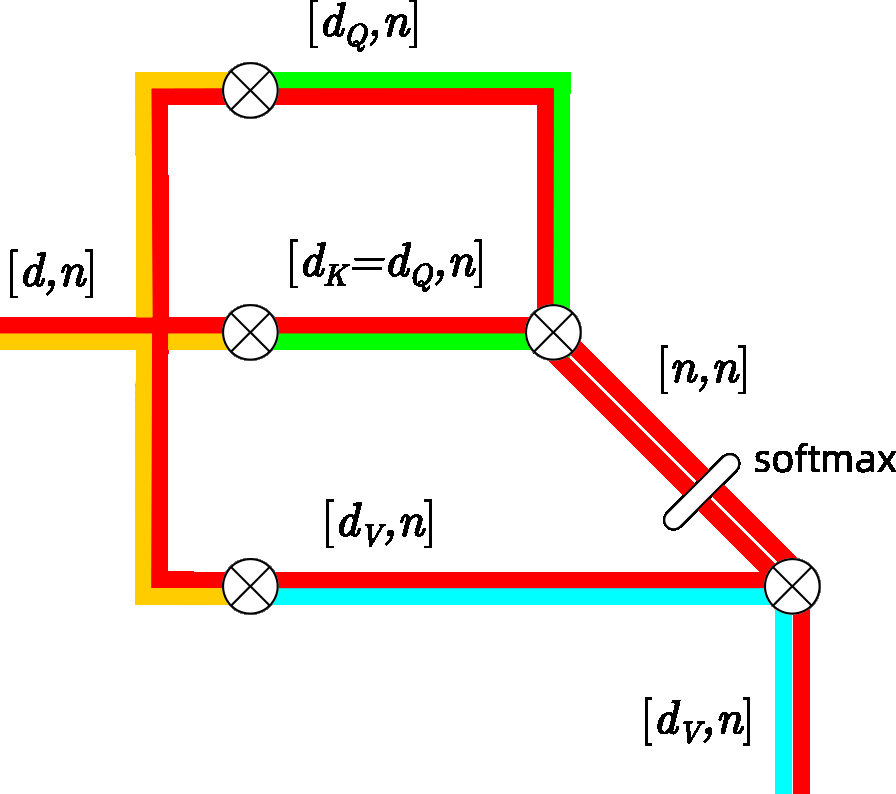
\includegraphics[scale=0.4]{self-attention-string-diagram-3.png}}}
\end{equation}
大家应该记得，在线性代数里，一个 $m \times n$ 的矩阵 乘以 $n \times l$ 的矩阵，给出 $m \times l$ 的矩阵，夹在中间的 $n$ 被 \textbf{消去} 了。 作为特例，$(1 \times n) \times (n \times 1) = 1$，这就是两个矢量之间的 dot product。 在我的图像里，夹在中间的绿色被消去了，但我错误地将绿色线画在外面，所以看不到这规律（我当时知道这规律，但我想不到它是可以图像化的，于是我的分析就停在了那里。）

后来我看到了 \cite{Abbott2024} 的论文，那瞬间才恍然大悟，原来我的图 (\ref{eqn:string-diagram2}) 跟 他们的图 是一样的，也就是 图 (\ref{eqn:attention-string-diagrams}) 的右下角。 他们不需要用颜色，而是将两条线在空间上「夹着」的维度消去。 而且这是对所有 tensor products 都适用的，那就是两个张量之间的 \textbf{缩并} (contraction), 也就是 TensorFlow 里面的 einsum（爱恩斯坦 求和约定）。\footnote{在图 (\ref{eqn:attention-string-diagrams}) 的右边，会看到有些 $\rightarrow$ 的终点没有任何东西，好像有些讯息消失了，其实这就是 tensor contraction，而讯息没有消失，可以看成是保留了在两条绳之间的空白部分。}

这件事的意义是： 代数上的对称性 可以用 string diagram 表示，而这些图可以根据一些特定的法则 做视觉上的 \textbf{变形} (string diagram rewriting)，保持 对称性的不变，而不需要写出 代数上的证明。 那些法则就是 symmetric monoidal categories (SMCs) 的组合法则。

【 岔开一点话题：如果大家懂一些 algebraic combinatorics，应该知道 \textbf{对称多项式} 有几种不同的 bases，例如 elementary $(e)$, monomial $(m)$, complete homogeneous $(h)$, power sum $(p)$, Schur $(s)$, forgotten $(f)$.  它们由 SMC 的生成元产生，而 \textbf{图重写} 对应于 多项式的 \textbf{基底变换}。暂时我还不清楚这个角度可以带来什么启发。】

这篇短文里我主要想讲的是： 我一直在学习 范畴逻辑理论 里面很旧、很基本的一些东西，但最近我的「研究」终于接触到 别的研究者 的「前沿」，这感觉非常良好。（当然，这是指数学方面的研究，在 AGI 方面，我觉得我已经算是专家。） 我想表达的是数学的神秘与奇妙，而这种「魔法」是有严谨的基础的，不是随意瞎扯出来的。

\printbibliography[heading=none]

\end{minipage}
\end{preview}

\end{document}
